230. \begin{figure}[ht!]
\center{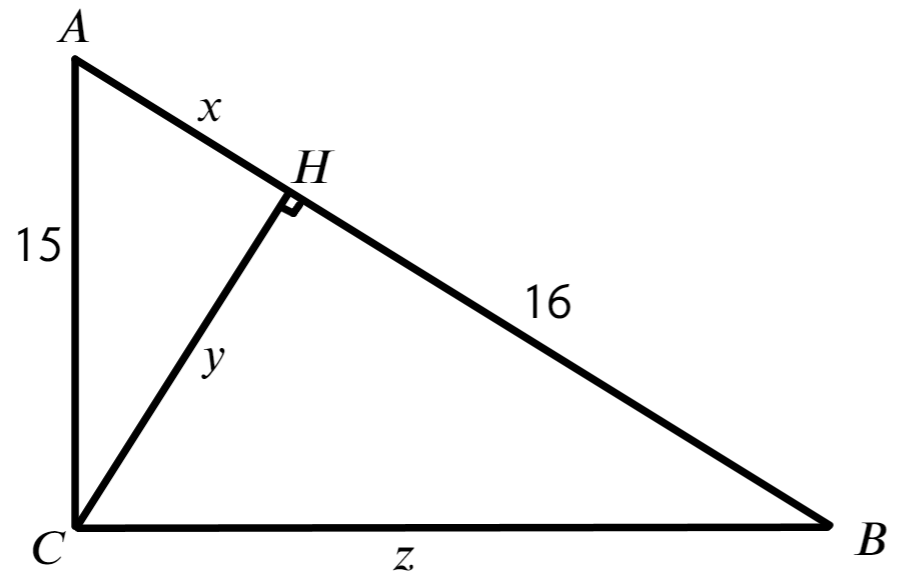
\includegraphics[scale=0.35]{g8-230.png}}
\end{figure}\\
Пусть $AH=x,\ CH=y,\ BC=z.$ Тогда из теорем Пифагора для прямоугольных треугольников $ACH,\ BCH$ и $ABC$ имеем систему уравнений $\begin{cases} x^2+y^2=225,\\ y^2+256=z^2,\\ z^2+225=(x+16)^2.\end{cases}$ Сложив все левые части и все правые, получим соотношение $2y^2+z^2+x^2+479=z^2+479+x^2+32x,\ 2y^2=32x,\ y^2=16x.$ Тогда $16x+x^2=225,\ x^2+16x-225=0,\ (x-9)(x+25)=0,\ x=9$см. Значит, $y^2=16\cdot9,\ y=4\cdot3=12$см. Тогда $S_{\Delta ABC}=\cfrac{1}{2}\cdot12\cdot(9+16)=150\text{ см}^2.$
ewpage
oindent
